\documentclass[conference]{IEEEtran}
\usepackage{cite}
\usepackage{amsmath}
\usepackage{newtxmath}
\usepackage{fontspec}
\setmainfont{texgyretermes}[Extension=.otf, UprightFont=*-regular,
  BoldFont=*-bold, ItalicFont=*-italic, BoldItalicFont=*-bolditalic]
\setmonofont{texgyrecursor}[Extension=.otf, UprightFont=*-regular,
  BoldFont=*-bold, ItalicFont=*-italic, BoldItalicFont=*-bolditalic]
\usepackage{booktabs}
\usepackage{array}
\usepackage{url}
\usepackage{tikz}
\usetikzlibrary{arrows.meta,positioning,automata,shapes.geometric,calc,fit,backgrounds}
\usepackage{pgfplots}
\pgfplotsset{compat=1.18}
\usepackage[hidelinks]{hyperref}
\setlength{\emergencystretch}{1em}

\begin{document}

\title{Federated Break-Glass EHR with a Unified\\Key-Lifecycle State Machine}

% Four authors in two rows of two.
\makeatletter
\newcommand{\linebreakand}{%
  \end{@IEEEauthorhalign}\hfill\mbox{}\par
  \mbox{}\hfill\begin{@IEEEauthorhalign}}
\makeatother

\author{
\IEEEauthorblockN{Ojas Thakurela}
\IEEEauthorblockA{Reg.\ No.\ 240911282\\
School of Computer Engineering\\
MIT, Manipal, India}
\and
\IEEEauthorblockN{Powel Lawrence Lewis}
\IEEEauthorblockA{Reg.\ No.\ 240911458\\
School of Computer Engineering\\
MIT, Manipal, India}
\linebreakand
\IEEEauthorblockN{Avaneeth Gowda L}
\IEEEauthorblockA{Reg.\ No.\ 240911368\\
School of Computer Engineering\\
MIT, Manipal, India}
\and
\IEEEauthorblockN{Nandini Taldar}
\IEEEauthorblockA{Reg.\ No.\ 240911356\\
School of Computer Engineering\\
MIT, Manipal, India}
}

\maketitle

% Abstract and keywords (W1). Every sentence ends with its source tag.
\begin{abstract}
Log-gated decryption exists as a generic primitive (accountable and transparent decryption), and break-glass schemes for health records exist; but in the works we compare, the log-gated schemes carry no patient revocation lifecycle, and the health-record break-glass schemes are not described as gating key release on a committed log entry.
% src: facts-F8#1, facts-F8#2, facts-F8#3, facts-F8#9, facts-F8#13, facts-F8#14, facts-F8#15, facts-F8#18, facts-F8#23
We implement a federated electronic health record prototype in which patient revocation, break-glass and expiry are signed, logged transitions of one key-lifecycle state machine over per-record keys, while consent is a patient-signed grant checked at read time when one is presented (status, window, signature), separate from the lifecycle state; revocation and expiry re-key the record in full, and opening break-glass rotates nothing.
% src: facts-F1#1, facts-F1#11, facts-F1#35, facts-F1#46, facts-F1#47, facts-F1#77, facts-F1#78
Following transparent decryption, the audit service holds two of four shares of each record's emergency key and releases them only after validating a signed, one-time Emergency Assertion bound to the record and committing a hash-chained log entry.
% src: facts-F8#3, facts-F2#34, facts-F2#36, facts-F2#45, facts-F2#50, facts-F2#51
Emergency search, derived from that key, ends at the expiry rotation.
% src: facts-F3#51, facts-F3#53, facts-F3#54
On a simulated federation with synthetic data, all eleven security claims hold in a live run, and PyShark checks see the audit commit on the wire before the shares.
% src: facts-F4#1, facts-F5#8, facts-live#12, facts-F6#43, facts-F6#49
Limitations: revocation is forward-only; expiry is server-enforced, not cryptographic; the access structure is not full CP-ABE (not collusion-resistant); the audit service is trusted (no proofs of presence or extension) and is a single point of availability, as the home authority's share replaces only a lost custodian share; and ``no plaintext on the wire'' holds only under TLS.
% src: facts-F5#16, facts-F1#54, facts-F3#41, facts-F2#59, facts-F5#11, facts-F2#62, facts-F2#63, facts-F6#6
\end{abstract}

\begin{IEEEkeywords}
Electronic health records, break-glass access, transparent decryption, threshold secret sharing, key rotation, audit logging, traffic analysis
\end{IEEEkeywords}

% Section I (W1). Every technical sentence ends with its source tag.
\section{Introduction}\label{sec:intro}

In an emergency a clinician may need records that the normal access policy does not grant, and static access control handles this poorly in health care, where break-glass is often bolted on ad hoc~\cite{brucker2009extending}.
% src: facts-F8#6
Hospital systems add a break-the-glass override and record its use for later review~\cite{ferreira2006break}; once records are encrypted, the override must also release a key~\cite{brucker2010abe,li2013phr}.
% src: facts-F8#7, facts-F8#9, facts-F8#15

Log-gated decryption is established: in accountable and transparent decryption a key, or a share of one, is used only once the request is in a log~\cite{ryan2017accountable,kroll2018accountable,cheval2023transparency}, and Kroll et al.\ name hospital emergencies as an application~\cite{kroll2018accountable}.
% src: facts-F8#1, facts-F8#2, facts-F8#3
Break-glass for health records is established too, at the policy layer, where consent gets a lifecycle but is enforced in software~\cite{muslim2026consent}, and with keys~\cite{brucker2010abe,deoliveira2020breakglass,yang2018libac,romel2025patient}, but none of those we examined is described as gating key release on a log entry.
% src: facts-F8#17, facts-F8#9, facts-F8#13, facts-F8#14, facts-F8#18
In the works we compare (Table~\ref{tab:related}), the log-gated schemes have no patient revocation lifecycle, so none joins log-gated release to consent and revocation.
% src: facts-F8#23

This paper builds that combination and tests it.
% src: facts-F8#24
Each record is encrypted under its own data-encryption key (DEK) and moves among four lifecycle states (\texttt{GRANTED}, \texttt{REVOKED}, \texttt{EMERGENCY\_OPEN}, \texttt{EXPIRED}) by seven legal transitions, each an ECDSA-signed event.
% src: facts-F3#25, facts-F1#1, facts-F1#11, facts-F1#3, facts-F1#28
Break-glass reconstructs a per-record emergency key from three of four Shamir shares, two of which belong to the audit service, so every unlock needs the audit service.
% src: facts-F2#33, facts-F2#34, facts-F2#36
The federation is simulated: two facilities, two attribute authorities, an audit service and a key custodian on one machine, with synthetic data.
% src: facts-F4#1, facts-F5#8

Our running scenario is an unconscious patient who arrives at an out-of-network clinic (Facility~B), while the patient's records sit encrypted in a shared store and the patient's home facility is Facility~A.
The clinician reads the patient's name and date of birth from an ID card, finds the patient in the clinician portal and declares an emergency with a signed Emergency Assertion.
The audit service logs the request and only then releases its two shares; with a third share, from the clinician's key agent (the key custodian) or the patient's home authority, the facility rebuilds the record's emergency key and opens the record.
The clinician reads and searches the patient's records across facilities, and when the time window ends the record is re-keyed with no administrator action.
% src: facts-F4#1, facts-F9#7, facts-F2#33, facts-F2#34, facts-F2#36, facts-F2#50, facts-F1#47, facts-F1#55, facts-F3#51
We claim the combination, implemented, and not any of its parts:
% src: facts-F8#24
\begin{itemize}
\item \emph{One signed, logged key lifecycle.}
Patient revocation, break-glass and expiry are signed transitions of one state machine over per-record DEKs; consent is a patient-signed grant checked at read time when one is presented (status, window, signature), separate from the lifecycle state, which it does not move.
% src: facts-F1#9, facts-F1#11, facts-F1#35, facts-F1#46, facts-F1#77, facts-F1#78
Revocation and expiry rotate the DEK, the policy root, the emergency key with its shares and the search index; opening break-glass rotates nothing (Section~\ref{sec:lifecycle}).
% src: facts-F1#36, facts-F1#40, facts-F1#47
\item \emph{Transparent-decryption-style log gating for federated break-glass.}
The audit service releases its two shares only after validating a signed, one-time Emergency Assertion bound to the record and committing a hash-chained log entry (Section~\ref{sec:breakglass}).
% src: facts-F2#6, facts-F2#45, facts-F2#50, facts-F2#51, facts-F8#3
\item \emph{Emergency-scoped search.}
Search tokens derive from the emergency key, so search works only during a live emergency session, and old tokens stop matching after expiry rotation.
% src: facts-F3#51, facts-F3#53, facts-F3#54
\item \emph{Evidence.}
Negative security tests back eleven claims, C1--C11; all 35 system tests tagged to them pass in a live run on the evaluated version of the code (Sections~\ref{sec:security} and~\ref{sec:eval}), as test outcomes, not proofs; the mutation evidence for them is partial (Section~\ref{sec:security}).
% src: facts-live#12, facts-F5#22
PyShark wire checks see the audit service's database commit before the release response that carries the shares (Section~\ref{sec:traffic}).
% src: facts-F6#43, facts-F6#47, facts-F6#49
\end{itemize}
We are weaker than the transparent-decryption literature in two ways: our log is a plain hash chain held by a trusted audit service, with no proofs of presence or extension, and we give no formal model (Section~\ref{sec:limits}).
% src: facts-F8#3, facts-F8#24, facts-F2#59

% Section II (W1). Every technical sentence ends with its source tag.
% Rival descriptions come from facts-F8 only; the "this work" row of
% Table tab:related comes from facts-live/F1/F2/F3 (see paper/data/make_related.py).
\section{Related Work}\label{sec:related}

Table~\ref{tab:related} compares the closest work with ours, group by group.
% src: facts-F8#23

% Generated by paper/data/make_related.py from paper/notes/facts-F8.md
% (rival rows) and facts-live/F1/F2/F3/F8 (this-work row). Do not edit by hand.
\begin{table}[t]
\centering
\caption{Comparison with related work (legend and notes below the table).}
\label{tab:related}
\footnotesize
\setlength{\tabcolsep}{2.4pt}
\begin{tabular}{@{}lcccccccc@{}}
\toprule
Work & CE & LG & BG & LC & TB & ES & FP & IMP \\
\midrule
Kroll et al.~\cite{kroll2018accountable} & $\checkmark$ & $\checkmark$ & $\circ$ & -- & ? & -- & $\circ$ & $\checkmark$ \\ % src: facts-F8#1
Ryan~\cite{ryan2017accountable} & $\checkmark$ & $\checkmark$ & -- & -- & -- & -- & $\circ$ & -- \\ % src: facts-F8#2
Cheval et al.~\cite{cheval2023transparency} & $\checkmark$ & $\checkmark$ & -- & -- & -- & -- & $\checkmark$ & $\circ$ \\ % src: facts-F8#3
Larch~\cite{dauterman2023larch} & $\checkmark$ & $\checkmark$ & -- & -- & -- & -- & ? & $\checkmark$ \\ % src: facts-F8#4
Li et al.~\cite{li2025accountable} & $\checkmark$ & $\checkmark$ & ? & -- & -- & -- & $\checkmark$ & $\checkmark$ \\ % src: facts-F8#5
\midrule
Brucker, Petritsch~\cite{brucker2009extending} & -- & -- & $\checkmark$ & -- & ? & -- & ? & ? \\ % src: facts-F8#6
Ferreira et al.~\cite{ferreira2006break} & -- & -- & $\checkmark$ & -- & ? & -- & ? & $\checkmark$ \\ % src: facts-F8#7
Marinovic et al.~\cite{marinovic2011rumpole} & -- & ? & $\checkmark$ & ? & ? & -- & ? & ? \\ % src: facts-F8#8
\midrule
Brucker et al.~\cite{brucker2010abe} & $\checkmark$ & ? & $\checkmark$ & ? & ? & -- & ? & ? \\ % src: facts-F8#9
Zhang et al.~\cite{zhang2016password} & $\checkmark$ & -- & $\checkmark$ & ? & ? & -- & ? & ? \\ % src: facts-F8#10
Scafuro~\cite{scafuro2019breakglass} & $\checkmark$ & $\circ$ & $\checkmark$ & -- & -- & -- & $\checkmark$ & -- \\ % src: facts-F8#11
de Oliveira et al.~\cite{deoliveira2019redalert} & $\checkmark$ & -- & $\checkmark$ & $\circ$ & $\checkmark$ & -- & -- & -- \\ % src: facts-F8#12
de Oliveira et al.~\cite{deoliveira2020breakglass} & $\checkmark$ & -- & $\checkmark$ & $\circ$ & $\checkmark$ & -- & $\checkmark$ & $\checkmark$ \\ % src: facts-F8#13
LiBAC~\cite{yang2018libac} & $\checkmark$ & -- & $\checkmark$ & -- & ? & -- & $\checkmark$ & $\checkmark$ \\ % src: facts-F8#14
\midrule
Li et al.~\cite{li2013phr} & $\checkmark$ & -- & $\checkmark$ & $\circ$ & -- & -- & ? & $\checkmark$ \\ % src: facts-F8#15
\midrule
Yang, Ma~\cite{yang2016timing} & $\checkmark$ & -- & -- & $\circ$ & $\checkmark$ & $\checkmark$ & $\checkmark$ & $\circ$ \\ % src: facts-F8#16
\midrule
Muslim, Gr\'egoire~\cite{muslim2026consent} & -- & -- & $\checkmark$ & $\circ$ & ? & -- & $\circ$ & $\checkmark$ \\ % src: facts-F8#17
Romel et al.~\cite{romel2025patient} & $\checkmark$ & -- & $\checkmark$ & $\circ$ & $\checkmark$ & -- & $\circ$ & $\checkmark$ \\ % src: facts-F8#18
\midrule
\textbf{This work} & $\checkmark$ & $\checkmark^{a}$ & $\checkmark$ & $\circ^{b}$ & $\checkmark^{c}$ & $\checkmark$ & -- & $\checkmark$ \\ % src: facts-live#12, facts-F1#11, facts-F1#35, facts-F1#54, facts-F1#77, facts-F1#78, facts-F2#50, facts-F2#59, facts-F3#53, facts-F8#3
\bottomrule
\end{tabular}
\par\vspace{3pt}
{\raggedright CE: keys, not a policy check, decide access; LG: key release
gated on a log entry; BG: break-glass; LC: consent and revocation in one
lifecycle; TB: time-boxed expiry; ES: emergency-scoped or time-limited
search; FP: formal proof or model; IMP: implementation. $\checkmark$ yes,
$\circ$ partial, -- no, ? not determined from what we read. Our row: live
run on \texttt{57a1a8c}.
% src: facts-live#12
$^{a}$Trusted hash chain, no log proofs.
% src: facts-F2#59, facts-F8#3
$^{b}$Revocation is a transition; consent is a signed grant checked at
read time when presented, outside the lifecycle.
% src: facts-F1#11, facts-F1#35, facts-F1#77, facts-F1#78
$^{c}$Server-enforced, not cryptographic.\par}
% src: facts-F1#54
\end{table}


\textit{Accountable and transparent decryption.}
Ryan~\cite{ryan2017accountable} proposes accountable decryption, in which a trusted hardware device decrypts only after the request is entered in a log whose untrusted maintainer gives proofs of presence and extension.
% src: facts-F8#2
Cheval, Moreira and Ryan~\cite{cheval2023transparency} formally verify transparent decryption in ProVerif: trustees hold shares of the decryption key and use them only if the Merkle-tree log proofs verify.
% src: facts-F8#3
Kroll et al.~\cite{kroll2018accountable} mediate every access through an approver and a threshold of decryption authorities, and the other parties do not proceed until an auditor certifies that the access is in its publicly verifiable log.
% src: facts-F8#1
They name hospital emergencies as an application: an unpredictable set of staff may suddenly need a patient's records, and the audit record lets internal reviewers check afterwards that the access was not abused~\cite{kroll2018accountable}.
% src: facts-F8#1
Larch~\cite{dauterman2023larch} applies the log-as-secret-holder pattern to authentication, and Li et al.~\cite{li2025accountable} give formal definitions of accountable decryption and a TEE-assisted construction.
% src: facts-F8#4, facts-F8#5
Transparent decryption is the primitive we instantiate: our logger holds two of four emergency-key shares, checks a signed Emergency Assertion before it commits, and sits inside a revocation and expiry lifecycle.
% src: facts-F8#1, facts-F8#3, facts-F2#34, facts-F2#36, facts-F2#45, facts-F1#47
Our log is weaker than all of these: a trusted hash chain, not publicly verifiable, with no proofs and no formal model.
% src: facts-F8#1, facts-F8#3, facts-F2#59

\textit{Break-glass access control.}
Ferreira et al.~\cite{ferreira2006break} add a break-the-glass policy with non-repudiation of its use to the access-control model of a hospital EMR, while Brucker and Petritsch~\cite{brucker2009extending} and Marinovic et al.~\cite{marinovic2011rumpole} build break-glass into access-control models.
% src: facts-F8#6, facts-F8#7, facts-F8#8
These are policy checks in software; in ours, keys and the threshold gate decide access, and the log entry precedes key release.
% src: facts-F8#6, facts-F8#7, facts-F4#19, facts-F2#51

\textit{Cryptographic break-glass.}
Brucker et al.~\cite{brucker2010abe} add break-glass to ABE-based information sharing, LiBAC~\cite{yang2018libac} lets an emergency override a file's ABE policy in healthcare IoT, and Zhang et al.~\cite{zhang2016password} let a password holder obtain a decryption key from a key generation centre that is held accountable for abuse.
% src: facts-F8#9, facts-F8#14, facts-F8#10
Scafuro~\cite{scafuro2019breakglass} builds encryption breakable exactly once, detectably, from hardware tokens, as a feasibility result.
% src: facts-F8#11
De Oliveira et al.\ limit emergency access to the task at hand~\cite{deoliveira2019redalert}, or to each team's period of care across institutions using signed access tokens and revocation by a trusted master authority and storage provider, without re-encrypting data~\cite{deoliveira2020breakglass}.
% src: facts-F8#12, facts-F8#13
None gates key release on a committed log entry (Scafuro's break is detectable, not log-gated), and our expiry re-keys the record instead of trusting a provider to block access; several, however, have formal analyses we lack.
% src: facts-F8#9, facts-F8#10, facts-F8#11, facts-F8#12, facts-F8#13, facts-F8#14, facts-F1#39

\textit{Encrypted PHR sharing.}
Li et al.~\cite{li2013phr} share personal health records on semi-trusted servers with multi-authority ABE, with multiple security domains, on-demand user and attribute revocation, and break-glass access in emergencies.
% src: facts-F8#15
We keep their patient-centric, multi-authority setting, but release the emergency key only through an audit-logged threshold, and the emergency ends with a rotation.
% src: facts-F8#15, facts-F2#36, facts-F1#55

\textit{Time-limited search.}
Yang and Ma~\cite{yang2016timing} let patients delegate keyword search and decryption rights over their records for a controlled period.
% src: facts-F8#16
This is prior art; we only derive emergency search tokens from the emergency key, so search ends at the expiry rotation, an engineering choice.
% src: facts-F8#16, facts-F3#51, facts-F3#54

\textit{Consent at the policy layer.}
Muslim and Gr\'egoire~\cite{muslim2026consent} validate consent directives before activation in XACML, add bounded break-the-glass access logged for post-hoc review, and argue that consent needs a lifecycle of creation, activation, revocation and expiration; their enforcement is ``logical rather than cryptographic''.
% src: facts-F8#17
We realise revocation and expiration by re-keying, while consent stays a patient-signed grant checked at read time; their ``pre-commit'' commits a policy, not a log entry.
% src: facts-F8#17, facts-F1#47, facts-F1#77, facts-F1#78
Romel et al.~\cite{romel2025patient} keep encrypted records off-chain, with patient-signed, time-bounded permissions on a public chain and keys distributed by public-key wrapping; revocation flips an on-chain flag, and re-keying is a separate, optional workflow.
% src: facts-F8#18
They also support emergency access: two registered emergency physicians co-sign a request that expires after two hours and is emitted as an on-chain event; that grant is logged, but key release goes through a separate, design-only HSM-backed guardian, not gated on the log, whereas ours needs the audit service's shares.
% src: facts-F8#18, facts-F2#36

\section{Threat Model and Goals}\label{sec:threat}

\textbf{Assets.} In priority order: protected health information (PHI) in plaintext, per-record data-encryption
keys (DEKs), each record's emergency key, attribute keys, audit-chain
integrity, and metadata, which we do not claim to hide. % src: facts-F5#4

\textbf{Adversaries.} Each of four adversaries is modeled separately. % src: facts-F5#2
\emph{(A) The shared store}, honest-but-curious or fully dumped, sees all
ciphertext, wrapped keys and the coded search index, but never plaintext or an
unwrapped key; it learns access patterns, sizes and metadata (e.g., that a
break-glass occurred), never content. % src: facts-F5#13, facts-F5#14, facts-F4#25
\emph{(B) A compromised facility} can forge requests, present the
certificates it holds and replay captured messages; it reads what its own keys
authorize, but cannot break glass alone, since reconstruction needs three of
four shares and two are held only by the audit service. % src: facts-F5#15, facts-F5#16, facts-F2#36
\emph{(C) A rogue attribute authority} mints keys for its own namespace and,
as a patient's home authority, holds share~2, which with the custodian's
share~1 reconstructs nothing; it can, however, mint that patient's
\texttt{owner} key, so protection is partial. % src: facts-F5#17, facts-F5#18, facts-F5#12
\emph{(D) Colluding clinicians} who pool attribute keys are \emph{not}
stopped: our Shamir-over-policy-tree structure is not collusion-resistant.
% src: facts-F5#19
No adversary is an on-path network attacker; ``no plaintext on the wire'' is
a goal of the TLS profile only (Section~\ref{sec:traffic}). % src: facts-F5#21, facts-F6#5, facts-F4#33

\textbf{Trust assumptions.} AES-256-GCM, ECDSA, SHA-256, HKDF and Shamir
sharing are assumed sound. % src: facts-F5#5
Four parties are trusted, not modeled as adversaries. % src: facts-F5#21, facts-F5#6, facts-F4#31
\emph{The audit service} holds its own plain hash chain: tampering with stored
entries is detected, but a compromised audit service could release its shares
without a durable entry or show different chains to different parties, so
the log gate holds against everyone except the audit service itself. % src: facts-F5#9, facts-F2#59
\emph{The Key Custodian} is one shared process acting as every subject's key
agent: it holds every synthetic persona's signing key, PRE key, credentials
and share~1, and signs on their behalf, so its compromise lets an attacker
act as any persona. % src: facts-F4#14, facts-F5#10
\emph{The emergency timer}, a simulated HSM realized as a per-facility
signing key and monitor thread, could decline to expire a key; because expiry
is a signed, logged rotation, this is tamper-evident, not
prevented. % src: facts-F5#6, facts-F1#34, facts-F2#83
\emph{The PKI root} key, held only at bootstrap, is a single point of
trust. % src: facts-F4#31
Rate limiting, MFA and session threats are out of scope. % src: facts-F5#8

\textbf{Goals.} The goals are eleven claims; system-level tests decide each
claim's status (Section~\ref{sec:security}). % src: facts-F5#22, facts-F5#26, facts-live#13
\textbf{C1}~A revoked user cannot decrypt after re-wrap. % src: facts-live#13
\textbf{C2}~Break-glass fails closed when the audit service cannot commit. % src: facts-live#13
\textbf{C3}~A single share, including the audit service's, cannot open a record. % src: facts-live#13
\textbf{C4}~Search capability does not survive the emergency's expiry. % src: facts-live#13
\textbf{C5}~A tampered audit entry is detected by chain verification. % src: facts-live#13
\textbf{C6}~An illegal state transition is rejected. % src: facts-live#13
\textbf{C7}~A transition event with an invalid signature is rejected. % src: facts-live#13
\textbf{C8}~A replayed emergency assertion is rejected, not re-executed. % src: facts-live#13
\textbf{C9}~An authenticated but unauthorised caller is denied before any
crypto or DB work (BOLA). % src: facts-live#13
\textbf{C10}~An expired or revoked credential fails validation and releases no
key. % src: facts-live#13
\textbf{C11}~A patient login alone never releases a DEK. % src: facts-live#13
BOLA in C9 is broken object-level authorization. In C1, re-wrap is a full rotation to a policy that excludes the revoked
clinician; in C3, whose text predates the 3-of-4 split, the audit service's two
shares together are one short of the threshold. % src: facts-F1#37, facts-F5#58, facts-F2#36, facts-live#13

\textbf{Confidentiality, integrity, availability.} Confidentiality is the aim
of C1, C3, C4, C9, C10 and C11 and of the TLS-only wire goal; integrity of
C5--C8. Availability is deliberately subordinate: every control fails
closed, so an unavailable audit service blocks break-glass
(Section~\ref{sec:limits}, item~8). % src: facts-live#13, facts-F2#62, facts-F2#63

\section{System Overview}\label{sec:overview}

\begin{figure}[t]
\centering
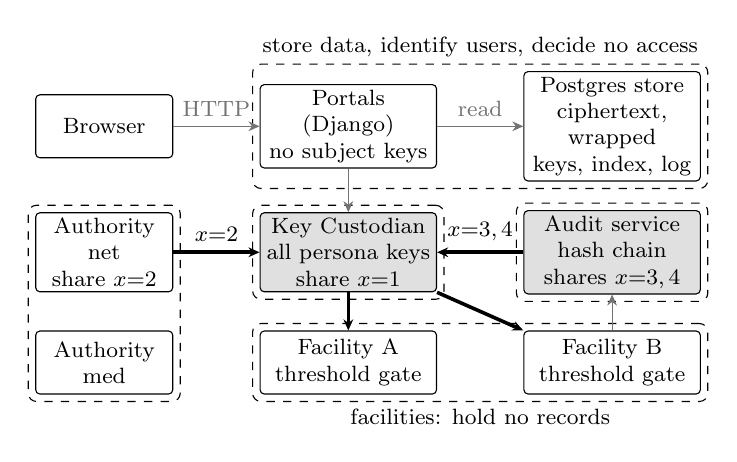
\begin{tikzpicture}[
  font=\footnotesize,
  >={Stealth[length=4pt,width=3.5pt]},
  comp/.style={draw, rounded corners=1.5pt, align=center, inner sep=2pt,
    minimum height=0.8cm, text width=#1},
  comp/.default=2.1cm,
  trusted/.style={fill=black!12},
  keyedge/.style={->, line width=1.3pt},
  aux/.style={->, black!55},
  bnd/.style={draw, dashed, rounded corners=3pt, inner sep=2.5pt},
]
% row 0: outside the key path
\node[comp=1.6cm] (br) at (0.85,0) {Browser};
\node[comp]       (po) at (3.95,0) {Portals (Django)\\no subject keys};
\node[comp]       (st) at (7.3,0) {Postgres store\\ciphertext, wrapped\\keys, index, log};
% row 1: key holders
\node[comp=1.6cm] (an) at (0.85,-1.6) {Authority net\\share $x{=}2$};
\node[comp, trusted] (cu) at (3.95,-1.6) {Key Custodian\\all persona keys\\share $x{=}1$};
\node[comp, trusted] (au) at (7.3,-1.6) {Audit service\\hash chain\\shares $x{=}3,4$};
% row 2
\node[comp=1.6cm] (am) at (0.85,-3.0) {Authority med};
\node[comp]       (fa) at (3.95,-3.0) {Facility A\\threshold gate};
\node[comp]       (fb) at (7.3,-3.0) {Facility B\\threshold gate};
% trust boundaries
\begin{scope}[on background layer]
  \node[bnd, fit=(po)(st), label={[yshift=-1pt]above:{store data, identify users, decide no access}}] {};
  \node[bnd, fit=(an)(am)] {};
  \node[bnd, fit=(fa)(fb), label={[yshift=1pt]below:{facilities: hold no records}}] {};
  \node[bnd, fit=(cu)] {};
  \node[bnd, fit=(au)] {};
\end{scope}
% non-key traffic
\draw[aux] (br) -- node[above] {HTTP} (po);
\draw[aux] (po) -- node[above] {read} (st);
\draw[aux] (po) -- (cu);
\draw[aux] (fb) -- (au);
% key path
\draw[keyedge] (an) -- node[above] {$x{=}2$} (cu);
\draw[keyedge] (au) -- node[above] {$x{=}3,4$} (cu);
\draw[keyedge] (cu) -- (fa);
\draw[keyedge] (cu.south east) -- (fb.north west);
\end{tikzpicture}
\caption{Simulated federation; dashed boxes are trust boundaries, shaded
parties are trusted. Thick arrows carry emergency-key shares, sealed to a
facility's gate; share~2 is used only if share~1 is missing. Thin arrows:
portal to custodian by subject id, no keys; facility to audit, log append
and, at rotation, the new sealed shares~3,4. Not drawn: portal-to-facility
calls, rotation deposits to custodian and authority, Postgres, root CA.}
% src: facts-F4#43, facts-F2#85, facts-F4#10, facts-F4#12, facts-F4#20, facts-F4#22, facts-F5#9, facts-F5#10
\label{fig:components}
\end{figure}

The federation is simulated: two mock facilities, two attribute authorities,
an audit service, a Key Custodian, a PostgreSQL store and one Django process
serving the patient, clinician and admin portals run on one machine, as local
processes or as Docker Compose containers on one bridge, under one
self-signed PKI root that signs both facility CAs
(Fig.~\ref{fig:components}). % src: facts-F4#1, facts-F4#5, facts-F4#27, facts-F4#43
There is no health-information exchange and no FHIR/HL7 interface, and all records are
synthetic. % src: facts-F4#1, facts-F4#44, facts-F4#39
The emergency scenario assumes the patient can be identified
(Section~\ref{sec:limits}, item~7). % src: facts-F9#7

\textbf{Components.} Facility~A is the patient's home facility and Facility~B
the out-of-network one where the emergency happens; neither holds records, and
both read ciphertext from the shared store and run the policy engine and
threshold gate. % src: facts-F4#7
An \emph{attribute authority} issues credentials and attribute keys, and the
patient's \emph{home authority} is the one that issued the patient's
\texttt{owner} credential. % src: facts-F4#8, facts-F5#12
The \emph{Key Custodian} is the key agent of clinicians and patients.
% src: facts-F4#14
This build chooses a weighted 3-of-4 split of each emergency key: $x{=}1$ to the custodian, $x{=}2$ to the home authority
(always \texttt{authority-net} here), $x{=}3,4$ to
the audit service, so every set of three shares includes an audit
share. % src: facts-F4#10, facts-F4#11, facts-F2#36

\textbf{Trust boundaries.} Every service call carries a root-issued service
certificate and a signed one-time request envelope, checked before any route
code runs, and key-bearing facility routes admit only the custodian or
bootstrap. % src: facts-F4#16, facts-F4#15
Shares travel sealed to the facility's gate; the audit service releases its
shares only after validating the assertion and committing a log entry
(Section~\ref{sec:breakglass}). % src: facts-F4#12

\textbf{Identity and certificates.} One self-signed root signs every facility
CA, attribute authority and service certificate; its key is held only at
bootstrap and is a single point of trust. % src: facts-F4#27, facts-F4#31
Certificates are X.509 with ECDSA P-256; a clinician's is signed by their
facility CA. % src: facts-F4#28, facts-F4#29
Because both facility CAs chain to the same root, Facility~B can validate a
clinician enrolled at Facility~A, which cross-facility break-glass needs;
chain validation fails closed on any bad link. % src: facts-F4#27, facts-F4#30
Each attribute authority issues signed credentials in its own namespace and
releases an attribute key only against a valid, unrevoked, unexpired
credential. % src: facts-F4#8, facts-F4#32

\textbf{Discovery and identification.} Records live in one shared store, so
discovery is a patient-indexed lookup that returns record identifiers only,
not a search across facilities. % src: facts-F4#9
To find the patient, the clinician portal looks up a name, optionally with a
date of birth, in its own directory; ambiguous matches are listed and never
auto-selected, a lookup that cannot be audited is not shown, and identifying
a patient releases no key. % src: facts-F9#7, facts-F4#19

\textbf{What portals and Postgres may not do.} They store data and identify
users but never decide access. % src: facts-F4#19
The portal holds no subject key and sends every key-needing action to the
custodian, so a portal account alone decrypts nothing; its database roles
cannot write store tables, and its consent state is display data only. % src: facts-F4#20, facts-F4#21, facts-F4#22, facts-F4#23

\section{Key-Lifecycle State Machine}\label{sec:lifecycle}

Every record carries one lifecycle state, and every committed change of it is
a signed, replay-protected event checked by one state machine in
\texttt{src/lifecycle/} (Fig.~\ref{fig:states}, Table~\ref{tab:transitions}).
% src: facts-F1#1, facts-F1#3, facts-F1#11, facts-F1#21, facts-F1#46, facts-F1#75

% Key-lifecycle state diagram (W3). States and arrows are the four
% LifecycleState values and the seven LEGAL_TRANSITIONS pairs in
% src/lifecycle/state_machine.py; signers and rotation marks follow
% facts-F1#46. Edit together with paper/data/make_transitions.py.
\begin{figure}[t]
\centering
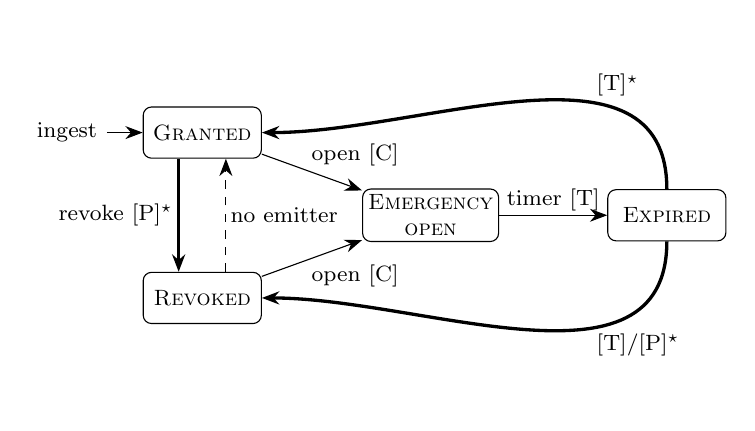
\begin{tikzpicture}[
    font=\footnotesize,
    >={Stealth[length=2.2mm]},
    st/.style={state, rectangle, rounded corners=3pt, minimum width=15mm,
      minimum height=6.5mm, inner sep=2pt, font=\footnotesize\scshape,
      align=center},
    rot/.style={->, very thick},
    plain/.style={->, thin},
    lbl/.style={font=\footnotesize, inner sep=1.5pt},
  ]
  \node[st, initial, initial text={ingest}, initial where=left]
    (G) at (0,1.05) {Granted};
  \node[st] (R) at (0,-1.05) {Revoked};
  \node[st] (E) at (2.9,0) {Emergency\\open};
  \node[st] (X) at (5.9,0) {Expired};
  % src: facts-F1#1, facts-F1#9, facts-F1#11

  \draw[rot] ([xshift=-3mm]G.south) -- node[lbl, left] {revoke [P]$^{\star}$}
    ([xshift=-3mm]R.north);
  % src: facts-F1#32, facts-F1#37
  \draw[plain, dashed] ([xshift=3mm]R.north) -- node[lbl, right] {no emitter}
    ([xshift=3mm]G.south);
  % src: facts-F1#35
  \draw[plain] (G) -- node[lbl, pos=0.45, above right] {open [C]} (E);
  \draw[plain] (R) -- node[lbl, pos=0.45, below right] {open [C]} (E);
  % src: facts-F1#30, facts-F1#36
  \draw[plain] (E) -- node[lbl, above] {timer [T]} (X);
  % src: facts-F1#33, facts-F1#53
  \draw[rot] (X.north) to[out=90, in=0] node[lbl, pos=0.35, above right]
    {[T]$^{\star}$} (G.east);
  \draw[rot] (X.south) to[out=-90, in=0] node[lbl, pos=0.35, below right]
    {[T]/[P]$^{\star}$} (R.east);
  % src: facts-F1#39, facts-F1#63, facts-F1#64, facts-F1#73
\end{tikzpicture}
\caption{Key-lifecycle states and the seven legal transitions. Signer:
[P]~patient, [C]~clinician, [T]~timer key; ``open'' is the break-glass unlock. Thick arrows ($\star$) carry a
full rotation; break-glass open rotates nothing. \textsc{Expired}$\to$\textsc{Revoked} is
timer- or patient-signed. The dashed
\textsc{Revoked}$\to$\textsc{Granted} pair is legal, but no code emits it.}
% src: facts-F1#11, facts-F1#35, facts-F1#36, facts-F1#46, facts-F1#47, facts-F1#73
\label{fig:states}
\end{figure}

% Generated by paper/data/make_transitions.py -- do not edit by hand.
% Pairs checked equal to lifecycle.state_machine.LEGAL_TRANSITIONS and facts-F1#46; signers checked against facts-F1#46.
\begin{table}[t]
\centering
\caption{Legal lifecycle transitions as shipped in \texttt{src/lifecycle/}. Any other pair raises \texttt{IllegalTransitionError} before signing. Signer ``Timer'' is the timer-service key.}  % src: facts-F1#11, facts-F1#19, facts-F1#33, facts-F1#73
\label{tab:transitions}
\footnotesize
\setlength{\tabcolsep}{2.5pt}
\renewcommand{\arraystretch}{1.1}
\begin{tabular}{@{}>{\raggedright\arraybackslash}p{0.14\columnwidth}>{\raggedright\arraybackslash}p{0.14\columnwidth}>{\raggedright\arraybackslash}p{0.29\columnwidth}>{\raggedright\arraybackslash}p{0.12\columnwidth}>{\raggedright\arraybackslash}p{0.23\columnwidth}@{}}
\toprule
From & To & Trigger & Signer & Key operation \\
\midrule
\textsc{Granted} & \textsc{Revoked} & Patient revokes & Patient & Full rotation$^{a}$ \\  % src: facts-F1#32, facts-F1#37, facts-F1#46
\textsc{Granted} & \textsc{EmOpen} & Break-glass; reason code required & Clinician & None$^{b}$ \\  % src: facts-F1#14, facts-F1#30, facts-F1#36, facts-F1#46, facts-F3#46
\textsc{Revoked} & \textsc{EmOpen} & As above & Clinician & None$^{b}$ \\  % src: facts-F1#36, facts-F1#46
\textsc{Revoked} & \textsc{Granted} & Legal; no code emits it & --- & None implemented \\  % src: facts-F1#35, facts-F1#46
\textsc{EmOpen} & \textsc{Expired} & Timer: $\mathit{now}\ge\mathit{expires\_at}$ & Timer & None; rotation follows \\  % src: facts-F1#33, facts-F1#46, facts-F1#53
\textsc{Expired} & \textsc{Granted} & Timer, once rotation is stored and shares deposited & Timer & Full rotation$^{a}$ before it \\  % src: facts-F1#39, facts-F1#46, facts-F1#63
\textsc{Expired} & \textsc{Revoked} & As above, if \textsc{Revoked} before; or patient revokes & Timer or Patient & Full rotation$^{a}$ \\  % src: facts-F1#12, facts-F1#46, facts-F1#64, facts-F1#73
\bottomrule
\end{tabular}
\par\smallskip
\parbox{\columnwidth}{\raggedright $^{a}$New DEK and re-encrypted record, new policy root, new emergency key with fresh 3-of-4 shares, re-derived search index.  % src: facts-F1#37, facts-F1#40, facts-F1#46
 \newline $^{b}$3-of-4 combine; DEK unwrapped and delivered by a KEM to the clinician's ElGamal key; nothing is re-keyed (Section~\ref{sec:breakglass}).  % src: facts-F1#36, facts-F3#46
 \newline \textsc{EmOpen} = \textsc{Emergency\_Open}.}
\end{table}


\subsection{States and Transitions}\label{sec:lifecycle-states}

The machine has exactly four states: \textsc{Granted}, \textsc{Revoked},
\textsc{Emergency\_Open} and \textsc{Expired}.
% src: facts-F1#1
A record enters \textsc{Granted} at ingest, which also creates its first
emergency wrapping of the data-encryption key (DEK) at generation~0.
% src: facts-F1#9, facts-F3#30
\textsc{Granted} is a baseline, not the result of a grant operation: consent
grants do not move lifecycle state, and the consent module does not wrap or
re-wrap records.
% src: facts-F1#35
The legal set is a frozen set of seven $(\mathit{from},\mathit{to})$ pairs;
self-transitions and \textsc{Granted}$\to$\textsc{Expired} are illegal, and
there is no premature-termination edge out of \textsc{Emergency\_Open}.
% src: facts-F1#11, facts-F1#13, facts-F1#15, facts-F1#16
ADR-0030 (Accepted) defined six of the pairs; this build adds
\textsc{Expired}$\to$\textsc{Revoked} under ADR-0058, which is still Proposed.
% src: facts-F1#12
\textsc{Revoked}$\to$\textsc{Granted} is legal, but no code in the repository
emits it.
% src: facts-F1#35
\textsc{Emergency\_Open} can be entered only from \textsc{Granted} or
\textsc{Revoked}, and such an event must carry a reason code from a closed
enumeration.
% src: facts-F1#14, facts-F1#2

Not every transition rotates keys.
% src: facts-F1#47
Revocation and expiry perform a full rotation; opening break-glass rotates
nothing.
% src: facts-F1#36, facts-F1#37, facts-F1#39
A full rotation decrypts the record with the old DEK, re-encrypts it under a
fresh DEK and a new policy identifier, recompiles the policy tree under a fresh
32-byte root secret, generates and splits a fresh emergency key, wraps the new
DEK under both at generation${}+1$, and re-derives the search tokens under the
new emergency key.
% src: facts-F1#40
Break-glass open instead reconstructs the emergency key from three of four
shares, unwraps the DEK and delivers it to the clinician; nothing in the store
is re-keyed (Section~\ref{sec:breakglass}).
% src: facts-F1#36, facts-F3#46
When the emergency ends, the record returns to the state it was claimed from,
so an emergency cannot undo a revocation.
% src: facts-F1#52, facts-F1#64

\subsection{Signed Transitions}\label{sec:lifecycle-signing}

A transition is a frozen \texttt{TransitionEvent} carrying an event id,
record id, from- and to-state, actor id, optional reason code, issue time,
nonce and signature; unknown fields are rejected and the nonce must be at
least 16~bytes.
% src: facts-F1#3, facts-F1#4, facts-F1#5
The signed bytes are a domain tag (\texttt{ehr/transition-event/v1}) followed
by every field but the signature, in a fixed order, each length-prefixed.
% src: facts-F1#27, facts-F3#14
The domain tag keeps a clinician's transition signature from verifying as
their emergency assertion.
% src: facts-F1#72
Signatures are ECDSA on P-256 with SHA-256; the event id comes from
\texttt{uuid4} and the nonce from \texttt{secrets}.
% src: facts-F1#28, facts-F1#29

Revocation is signed with the patient's key and break-glass open with the
clinician's key, both inside the custodian.
% src: facts-F1#30, facts-F1#32
The facility verifies the break-glass event against the clinician's
certificate, requires its record, actor and reason code to match the
assertion, and requires an issue time under 15\,min old (30\,s skew) on its
own clock (Section~\ref{sec:breakglass}).
% src: facts-F1#31, facts-F1#74
The expiry-side transitions are signed by a timer-service key, never by the
clinician's or the audit service's key, though a patient may also revoke a
record left in \textsc{Expired}; each facility process makes a fresh timer key.
% src: facts-F1#33, facts-F1#34, facts-F1#73

Illegal transitions fail closed before anything is signed:
\texttt{create\_\allowbreak transition\_\allowbreak event} calls
\texttt{validate\_\allowbreak transition} first,
which raises \texttt{Illegal\-Transition\-Error} for any pair outside the legal
set, so no event id, nonce or signature is produced.
% src: facts-F1#17, facts-F1#19
On receipt, \texttt{apply\_\allowbreak transition} verifies the signature, then re-checks
legality, then requires the event's from-state to equal the current state,
and finally consumes the event id, raising \texttt{Replayed\-Event\-Error} on
reuse.
% src: facts-F1#20, facts-F1#21, facts-F1#23
Because the signature is checked first, a tampered to-state surfaces as an
invalid signature, and a forged event cannot burn a legitimate id.
% src: facts-F1#20, facts-F1#22
The deployed facility backs the consumed-id store durably, so ids survive a
restart, and the record store adds its own compare-and-set on the stored
state (ADR-0050, Proposed).
% src: facts-F1#24, facts-F1#25

\subsection{Expiry}\label{sec:lifecycle-expiry}

Opening break-glass registers an emergency session with
$\mathit{expires\_at} = \mathit{now} + d$; the deployed default is
$d = 4$\,h, a caller may shorten but not extend it, and only one session per
record may be active.
% src: facts-F1#48, facts-F1#49, facts-F1#50, facts-F1#51
Expiry is enforced by the server, not by cryptography: once
$\mathit{now} \ge \mathit{expires\_at}$, the expiry manager refuses to hand out
the emergency key or admit a new join, even before the sweep runs
(Section~\ref{sec:limits}).
% src: facts-F1#53, facts-F1#54
A background monitor checks for due sessions every 0.5\,s, so no
administrator action is needed.
% src: facts-F1#55

The sweep first claims the session, so concurrent expirers cannot rotate
twice.
% src: facts-F1#57
It then signs \textsc{Emergency\_Open}$\to$\textsc{Expired} with the timer
key, runs the full rotation, and only after the rotation is stored and the new
shares are deposited signs the return to \textsc{Granted} or
\textsc{Revoked}.
% src: facts-F1#39, facts-F1#63
Each timer transition is written to the audit log first, with identifiers but
no key material, and then mirrored into the store by compare-and-set.
% src: facts-F1#60, facts-F1#61
A failed attempt is retried with backoff capped at 60\,s while access stays
closed, reusing the already-signed events and the first rotation plan, so in-process
it neither re-signs nor mints a second emergency key.
% src: facts-F1#45, facts-F1#58, facts-F1#59

For crash recovery this build chooses (ADR-0081, Proposed) to persist, when a
session opens, a row of identifiers that holds no key; if that write fails,
the session is not registered.
% src: facts-F1#66
At startup a facility reloads its own rows for records still in
\textsc{Emergency\_Open} or \textsc{Expired} as sessions with no emergency
key and $\mathit{expires\_at} = \mathit{now}$, so nobody can join them and
the next sweep expires them.
% src: facts-F1#67, facts-F1#68
The rotator then recovers the DEK through the record's policy, the same path
revocation uses; if the store already shows \textsc{Expired}, that event is
signed afresh but not logged again.
% src: facts-F1#69, facts-F1#70, facts-F1#76

\subsection{Access Structure: Shamir over a Policy Tree}\label{sec:lifecycle-access}

In place of CP-ABE, a hand-rolled access structure guards each record's DEK.
% src: facts-F3#3, facts-F3#34
A policy is a tree of \textsc{Leaf}, \textsc{And} and \textsc{Or} nodes,
with no general $k$-of-$n$ gate.
% src: facts-F3#32
It is compiled top-down from a fresh 32-byte root secret: an \textsc{And}
node with $m$ children Shamir-splits its incoming secret $m$-of-$m$, an
\textsc{Or} node passes the same secret to every child, and a leaf encrypts
its incoming secret with AES-256-GCM under an attribute key.
% src: facts-F3#33
The root secret is the DEK wrapping key; the wrapping's associated data binds
the record id, policy id and generation, so a wrapping cannot be moved to
another record or replayed as another generation.
% src: facts-F3#29, facts-F3#34
Attribute keys are symmetric 32-byte keys indexed by
(authority, attribute name, value), so the same \texttt{name:value} from
another authority does not open a leaf.
% src: facts-F3#36
Leaf ciphertexts carry no associated data and are therefore not bound to
their record, position or attribute.
% src: facts-F3#35
Every record's tree has the form
$\textsc{Or}(\mathit{clinical\ policy}, \mathit{owner}{:}\mathit{patient})$,
where the owner leaf belongs to the patient's home authority.
% src: facts-F3#40
Reconstruction runs bottom-up and raises \texttt{PolicyDeniedError} if the
root is unsatisfied; it never returns a partial or default secret.
% src: facts-F3#38

Shamir sharing works over $\mathrm{GF}(p)$ with $p = 2^{256}+297$, a
257-bit prime; the secret, prefixed with its 4-byte length and zero-padded,
is cut into 32-byte blocks, each one field element with its own random
polynomial and a 33-byte share element.
% src: facts-F3#17, facts-F3#22
Shares are not authenticated: a well-formed wrong share yields a wrong secret,
which the AES-GCM unwrap downstream detects.
% src: facts-F3#24
The same code splits each record's emergency key 3-of-4, with $x=1$ held by
the clinician custodian, $x=2$ by the home authority, and $x=3,4$ by the audit
service (ADR-0089, Proposed); Section~\ref{sec:breakglass} describes the gate
that combines them.
% src: facts-F1#41, facts-F3#49

This construction is not full CP-ABE.
% src: facts-F3#41
It is not collusion-resistant: two clinicians can pool attribute keys to
satisfy a policy that neither satisfies alone, which pairing-based CP-ABE
prevents.
% src: facts-F3#41
It has no security proof (Section~\ref{sec:security}).
% src: facts-F3#41
Attribute keys are also shared by every holder of an attribute and never
rotated, so revoking a credential stops future releases but does not take
back a key already held (Section~\ref{sec:limits}).
% src: facts-F3#37

\section{Break-Glass Protocol}\label{sec:breakglass}

% Break-glass message sequence (W4). Every arrow and box is a step in
% facts-F2 section G (fact 60) and the facts tagged per line below.
\begin{figure}[!t]
\centering
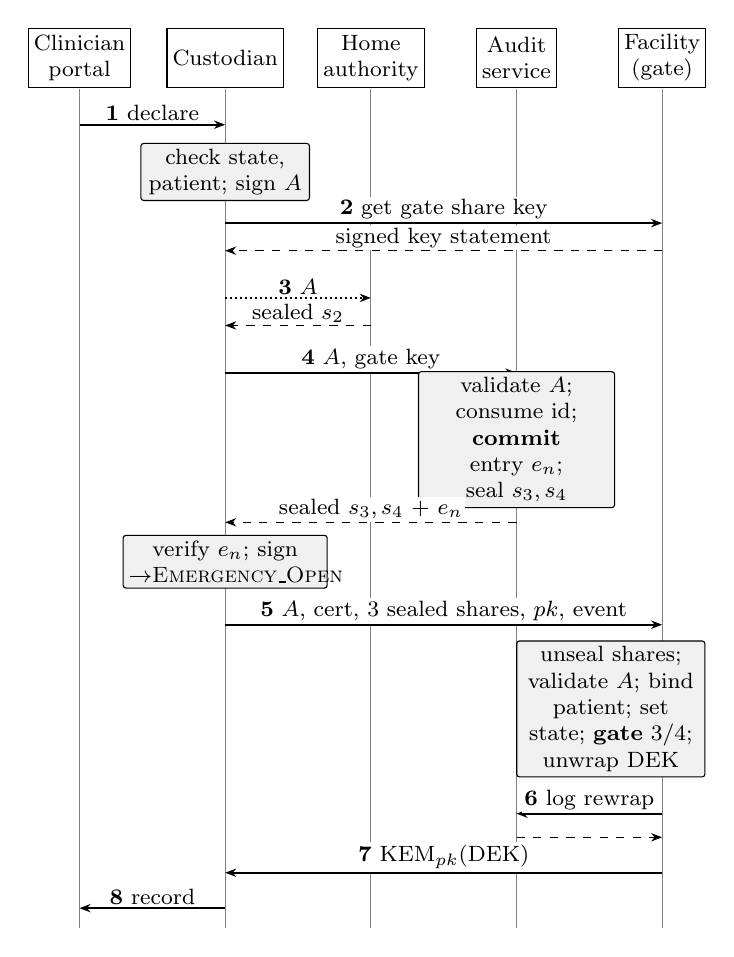
\begin{tikzpicture}[
  font=\footnotesize,
  >={Stealth[length=4pt]},
  head/.style={draw, fill=white, align=center, inner sep=2pt, minimum height=0.75cm},
  act/.style={draw, fill=gray!12, align=center, inner sep=2pt, rounded corners=1pt},
  msg/.style={->, thick},
  ret/.style={->, dashed},
  opt/.style={->, densely dotted, thick},
  lbl/.style={above, inner sep=1pt, fill=white},
  num/.style={font=\footnotesize\bfseries}
]
% lifelines
\def\xP{0} \def\xC{1.85} \def\xH{3.7} \def\xA{5.55} \def\xF{7.4}
\def\ybot{-11.05}
\foreach \x/\t in {\xP/{Clinician\\portal}, \xC/{Custodian}, \xH/{Home\\authority}, \xA/{Audit\\service}, \xF/{Facility\\(gate)}}{
  \draw[gray] (\x,-0.4) -- (\x,\ybot);
  \node[head] at (\x,0) {\t};
}
% 1  portal -> custodian (facts-F2#89)
\draw[msg] (\xP,-0.85) -- node[lbl]{\textbf{1} declare} (\xC,-0.85);
% custodian checks state and patient, signs the assertion (facts-F2#5, F2#17, F2#92)
\node[act, text width=2.0cm] at (\xC,-1.45) {check state, patient; sign $A$};
% 2  gate share key (facts-F2#60, F2#42)
\draw[msg] (\xC,-2.1) -- node[lbl]{\textbf{2} get gate share key} (\xF,-2.1);
\draw[ret] (\xF,-2.45) -- node[lbl]{signed key statement} (\xC,-2.45);
% 3  fallback: home authority, only if share 1 is lost (facts-F2#60-62)
\draw[opt] (\xC,-3.05) -- node[lbl]{\textbf{3} $A$} (\xH,-3.05);
\draw[ret] (\xH,-3.4) -- node[lbl]{sealed $s_2$} (\xC,-3.4);
% 4  audit release (facts-F2#50-53)
\draw[msg] (\xC,-4.0) -- node[lbl]{\textbf{4} $A$, gate key} (\xA,-4.0);
\node[act, text width=2.35cm] at (\xA,-4.85) {validate $A$;\\ consume id;\\ \textbf{commit} entry $e_n$;\\ seal $s_3,s_4$};
\draw[ret] (\xA,-5.9) -- node[lbl]{sealed $s_3,s_4$ + $e_n$} (\xC,-5.9);
% custodian verifies e_n, signs the transition (facts-F2#55, F2#60)
\node[act, text width=2.45cm] at (\xC,-6.4) {verify $e_n$; sign\\ $\to$\textsc{Emergency\_Open}};
% 5  present to the facility (facts-F2#60)
\draw[msg] (\xC,-7.2) -- node[lbl]{\textbf{5} $A$, cert, 3 sealed shares, $pk$, event} (\xF,-7.2);
% facility path: unseal, then validate (facts-F2#93, F2#67, F2#65)
\node[act, text width=2.25cm, anchor=north east] at (\xF+0.55,-7.4) {unseal shares; validate $A$; bind patient; set state; \textbf{gate} 3/4; unwrap DEK};
% 6  second log-before-release (facts-F2#57)
\draw[msg] (\xF,-9.6) -- node[lbl]{\textbf{6} log rewrap} (\xA,-9.6);
\draw[ret] (\xA,-9.9) -- (\xF,-9.9);
% 7  KEM delivery to the clinician's ElGamal key (facts-F2#65, F2#90)
\draw[msg] (\xF,-10.35) -- node[lbl]{\textbf{7} KEM$_{pk}$(DEK)} (\xC,-10.35);
\draw[msg] (\xC,-10.8) -- node[lbl]{\textbf{8} record} (\xP,-10.8);
\end{tikzpicture}
\caption{Cross-facility break-glass. $A$ is the Emergency Assertion, signed in
the custodian with the clinician's key; $s_i$ is the share at $x=i$. Step~3
(dotted) runs only when share~1 is lost. The audit service commits its entry
before it seals and returns shares 3 and 4 (step 4), and the facility logs
the re-wrap before delivering the DEK (step 6).}
% src: facts-F2#5, facts-F2#17, facts-F2#42, facts-F2#50, facts-F2#55, facts-F2#57, facts-F2#60, facts-F2#61, facts-F2#62, facts-F2#65, facts-F2#67, facts-F2#89, facts-F2#90, facts-F2#92, facts-F2#93
\label{fig:sequence}
\end{figure}

% 3-of-4 gate (a) and audit hash chain (b) (W4). One float, both labels.
\begin{figure}[!t]
\centering
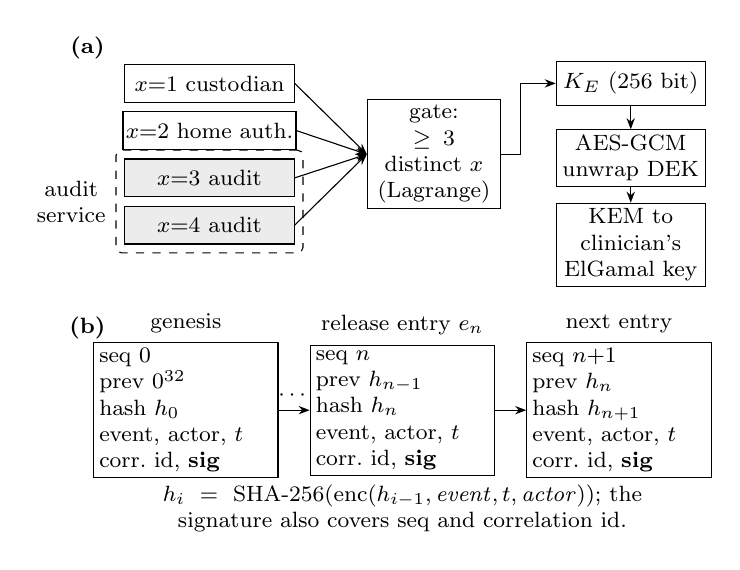
\begin{tikzpicture}[
  font=\footnotesize,
  >={Stealth[length=4pt]},
  sh/.style={draw, fill=white, minimum width=2.15cm, minimum height=0.48cm, inner sep=1pt},
  bx/.style={draw, fill=white, align=center, inner sep=2pt, minimum height=0.55cm}
]
% (a) shares by holder (facts-F2#33, F2#34)
\node[sh] (s1) at (0,0)     {$x{=}1$ custodian};
\node[sh] (s2) at (0,-0.6)  {$x{=}2$ home auth.};
\node[sh, fill=gray!15] (s3) at (0,-1.2) {$x{=}3$ audit};
\node[sh, fill=gray!15] (s4) at (0,-1.8) {$x{=}4$ audit};
\begin{scope}[on background layer]
  \node[draw, dashed, rounded corners=2pt, fit=(s3)(s4), inner sep=3pt,
        label={[font=\footnotesize, align=center]left:audit\\service}] {};
\end{scope}
% gate: no holder check, only ">= 3 distinct x" (facts-F2#37, F2#40)
\node[bx, text width=1.55cm] (g) at (2.85,-0.9) {gate:\\ $\ge 3$ distinct $x$\\ (Lagrange)};
\foreach \s in {s1,s2,s3,s4}{ \draw[->] (\s.east) -- (g.west); }
% key, unwrap, delivery (facts-F2#32, F2#65)
\node[bx, text width=1.75cm] (k) at (5.35,0)    {$K_E$ (256 bit)};
\node[bx, text width=1.75cm] (u) at (5.35,-0.95) {AES-GCM unwrap DEK};
\node[bx, text width=1.75cm] (d) at (5.35,-2.05) {KEM to clinician's ElGamal key};
\draw[->] (g.east) -- ++(0.25,0) |- (k.west);
\draw[->] (k) -- (u);
\draw[->] (u) -- (d);
\node[font=\footnotesize\bfseries] at (-1.55,0.45) {(a)};

% (b) hash chain (facts-F2#71-75)
\begin{scope}[yshift=-4.15cm]
\foreach \i/\x/\s/\p/\h in {0/-0.3/{$0$}/{$0^{32}$}/{$h_0$}, 1/2.45/{$n$}/{$h_{n-1}$}/{$h_n$}, 2/5.2/{$n{+}1$}/{$h_{n}$}/{$h_{n+1}$}}{
  \node[draw, fill=white, align=left, text width=2.2cm, inner sep=2pt] (e\i) at (\x,0)
    {seq \s\\ prev \p\\ hash \h\\ event, actor, $t$\\ corr.\ id, \textbf{sig}};
}
\node[font=\footnotesize, above=0pt of e0] {genesis};
\node[font=\footnotesize, above=0pt of e1] {release entry $e_n$};
\node[font=\footnotesize, above=0pt of e2] {next entry};
\draw[->] (e0.east) -- node[above, font=\footnotesize]{$\cdots$} (e1.west);
\draw[->] (e1.east) -- (e2.west);
\node[font=\footnotesize\bfseries] at (-1.55,1.05) {(b)};
\node[font=\footnotesize, align=center, text width=7.6cm] at (2.45,-1.25)
  {$h_i=\mathrm{SHA\text{-}256}(\mathrm{enc}(h_{i-1},\mathit{event},t,\mathit{actor}))$;
   the signature also covers seq and correlation id.};
\end{scope}
\end{tikzpicture}
\caption{(a) Weighted 3-of-4 gate. The gate checks no share holder, only for
three distinct $x$ values; that every qualifying set holds an audit share follows from the
placement of shares, not from a gate check. (b) Audit hash chain; entry $n$
is committed before shares 3 and 4 leave the audit service.}
% src: facts-F2#32, facts-F2#33, facts-F2#34, facts-F2#36, facts-F2#37, facts-F2#40, facts-F2#51, facts-F2#57, facts-F2#65, facts-F2#71, facts-F2#72, facts-F2#73, facts-F2#74
\label{fig:gate}\label{fig:chain}
\end{figure}


Break-glass moves a record from \textsc{Granted} or \textsc{Revoked} to
\textsc{Emergency\_Open}: a gate at the record's facility rebuilds the
record's emergency key from three of four Shamir shares and re-wraps the DEK
to the clinician (Fig.~\ref{fig:sequence}); opening rotates no key.
% src: facts-F1#14, facts-F1#36, facts-F2#16, facts-F2#65

\subsection{Emergency Assertion and Replay}

An Emergency Assertion $A$ carries a one-time identifier \texttt{assertion\_\allowbreak id};
patient, clinician and facility identifiers; a reason code from a closed
enumeration; \texttt{issued\_\allowbreak at}, \texttt{expires\_\allowbreak at}; a nonce of at least
128 bits; an optional digest binding the record and justification texts,
which the share holders require; and an ECDSA P-256 signature over all other
fields by the clinician's key, which never leaves the custodian.
% src: facts-F2#1, facts-F2#2, facts-F2#4, facts-F2#5, facts-F2#6, facts-F2#45, facts-F2#91
Validation fails closed at the first failing check, in order: signature;
certificate chain via a facility CA to the trusted root; clinician
identifier against the certificate CN; certificate not revoked; facility
identifier (at the holders, only federation membership); not expired; lifetime $\le 15$\,min and \texttt{issued\_\allowbreak at} at
most 30\,s in the future; then consumption of \texttt{assertion\_\allowbreak id}.
% src: facts-F2#7, facts-F2#18, facts-F2#46
Consumption runs last, so an invalid assertion cannot burn a legitimate
identifier, and the consumed store is a required argument that cannot be
omitted.
% src: facts-F2#9, facts-F2#10
The facility, the audit service and the home authority each validate $A$
against their own trust anchors and consume its identifier in their own
store (durable at the facility and audit service, in memory at the
authority), so a reused $A$ gets no shares 3 and 4 even after an authority
restart.
% src: facts-F2#14, facts-F2#26, facts-F2#27, facts-F2#45
No share holder checks that the record belongs to $A$'s patient; the
facility does, as does the custodian when it can load the record.
% src: facts-F2#12, facts-F2#47, facts-F2#92
The transition event and every signed service request also carry one-time
identifiers, and replay rejection (C8) holds in the live run.
% src: facts-F2#29, facts-F2#30, facts-live#8

\subsection{The Weighted 3-of-4 Gate}

The 256-bit emergency key $K_E$ wraps the DEK and is split with $k=3$,
$n=4$ over $\mathrm{GF}(p)$, $p=2^{256}+297$ (257 bits): the custodian holds
$x=1$, the home authority $x=2$, and the audit service $x=3,4$
(Fig.~\ref{fig:gate}a).
% src: facts-F2#32, facts-F2#33, facts-F2#34, facts-F2#38, facts-F3#30
The gate checks no share holder, only that three shares have distinct $x$;
that every qualifying set contains an audit share follows from the
distribution, since the two other holders have only two points between them.
% src: facts-F2#36, facts-F2#37
This build seals shares in transit: a KEM to the gate's
ElGamal key, whose signed statement holders verify, with record, $x$ and
recipient as associated data; the group is a 256-bit demonstration
parameter.
% src: facts-F2#41, facts-F2#42, facts-F2#43

\subsection{Commit-then-Release}

The audit service validates $A$, builds the log event from it, appends the
hash-chained entry inside one transaction, and only then seals shares 3
and 4 and returns them with the signed entry.
% src: facts-F2#50, facts-F2#51, facts-F2#53
A failed commit raises before the return and yields HTTP~503 with no share,
so there is no log entry, no key: C2 holds, and the wire shows the COMMIT
1.35\,ms before the response (Section~\ref{sec:traffic}).
% src: facts-F2#51, facts-F2#54, facts-live#2, facts-F6#49
The custodian checks the entry's signature, correlation identifier and
rising sequence number, and the facility logs the re-wrap before delivering
the DEK.
% src: facts-F2#55, facts-F2#57
The guarantee holds against everyone except the audit service, which is
trusted (Section~\ref{sec:limits}).
% src: facts-F2#59

The gate then unwraps the DEK and delivers it by a KEM to the clinician's
ElGamal key; the facility sees the plaintext DEK meanwhile.
% src: facts-F2#65, facts-F2#66, facts-F2#90
The home authority's share~2 covers a lost share~1 only, which the custodian
keeps in memory.
% src: facts-F2#62
It does not cover a custodian or audit outage, nor an audit restart, which
loses shares 3 and 4 for every record; by code reading, not observed, a
restarted audit service also has a new signing key and would fail its
startup chain check.
% src: facts-F2#63, facts-F2#64

\subsection{Hash Chain}

Each entry holds \texttt{seq}, \texttt{prev\_\allowbreak hash} and \texttt{entry\_\allowbreak hash},
the event type and metadata, the actor, a correlation identifier, a timestamp
and an ECDSA signature, with
$h_i=\mathrm{SHA\text{-}256}(\mathrm{enc}(h_{i-1},\mathit{event},t,\mathit{actor}))$
from a zero-hash genesis (Fig.~\ref{fig:chain}b).
% src: facts-F2#71, facts-F2#72, facts-F2#73, facts-F2#74
Verification checks signature, link, sequence and hash, and C5 holds.
% src: facts-F2#77, facts-live#5
Against truncation, a facility refuses an entry whose \texttt{seq} is not
above its stored mark; it compares sequence numbers only and verifies no
entry signature.
% src: facts-F2#79, facts-F2#81

\subsection{Expiry by Full Rotation}

The deployed window is 4\,h, which a caller may only shorten.
% src: facts-F2#20, facts-F2#21
At expiry a monitor signs \textsc{Emergency\_Open}$\to$\allowbreak\textsc{Expired},
runs a full rotation (new DEK, policy root and $K_E$, with a fresh 3-of-4
split to the same holders), and signs the return to the prior state
(Section~\ref{sec:lifecycle-expiry}); old shares then open nothing (C4).
% src: facts-F2#83, facts-F2#84, facts-F2#85, facts-F2#86, facts-live#4

\section{Security Analysis}\label{sec:security}

% Generated by paper/data/make_claims.py from paper/notes/live-claims-raw.txt.
% Do not edit by hand. Statements and statuses are verbatim from the live
% `python -m tests.security.claims --table` run (only LaTeX-escaped).
\begin{table}[!t]
\centering
\footnotesize
\setlength{\tabcolsep}{3pt}
\caption{Security claims C1--C11, from a live claims run. Status is computed from the system-level tests only; Sys./Mod.\ count the system- and module-level tests tagged with the claim.}
% src: facts-live#1, facts-live#2, facts-live#3, facts-live#4, facts-live#5, facts-live#6, facts-live#7, facts-live#8, facts-live#9, facts-live#10, facts-live#11, facts-live#12, facts-live#13
\label{tab:claims}
\begin{tabular}{@{}l p{0.64\columnwidth} l r r@{}}
\toprule
ID & Statement & Status & Sys. & Mod. \\
\midrule
C1 & A revoked user cannot decrypt after re-wrap & holds & 2 & 2 \\
C2 & Break-glass fails closed when the audit service cannot commit & holds & 1 & 1 \\
C3 & A single share, including the audit service's, cannot open a record & holds & 10 & 4 \\
C4 & Search capability does not survive the emergency's expiry & holds & 6 & 1 \\
C5 & A tampered audit entry is detected by chain verification & holds & 1 & 3 \\
C6 & An illegal state transition is rejected & holds & 1 & 1 \\
C7 & A transition event with an invalid signature is rejected & holds & 2 & 1 \\
C8 & A replayed emergency assertion is rejected, not re-executed & holds & 4 & 1 \\
C9 & An authenticated but unauthorised caller is denied before any crypto or DB work (BOLA) & holds & 3 & 0 \\
C10 & An expired or revoked credential fails validation and releases no key & holds & 4 & 2 \\
C11 & A patient login alone never releases a DEK & holds & 1 & 2 \\
\midrule
\multicolumn{3}{@{}l}{Total} & 35 & 18 \\
\bottomrule
\end{tabular}
\end{table}


Table~\ref{tab:claims} gives claims C1--C11 from a live run of the claim
registry.
% src: facts-live#13
A claim holds only when every system-level test tagged with it passed; a skip
makes it unverified, an expected failure ``fails today'', and module-level
outcomes never change a status.
% src: facts-F5#23, facts-F5#26
In the live run all eleven claims hold, with 35 of 35 system-level
tests passing and none skipped; these are outcomes of the tested cases, not
proofs (Table~\ref{tab:secprops}).
% src: facts-live#12

\subsection{Per-Claim Arguments}

\emph{C1:} after revocation through the facility endpoint, on the in-memory
store and on Postgres, the clinician cannot read.
% src: facts-live#13
Revocation re-keys through the expiry rotation (new emergency key, shares and
search index) and is forward-only.
% src: facts-F3#58, facts-F5#16
C1's test excludes the clinician by rotating to a policy that no longer
names their attribute; it does not cover a revoked holder whose attribute
the new policy still names, who still satisfies it with a kept key
(Section~\ref{sec:limits}, item~9).
% src: facts-F5#58, facts-F9#9
\emph{C2:} a test makes the audit commit fail
and gets no share; the append runs in one transaction that raises before any
share is returned.
% src: facts-live#13, facts-F2#51
\emph{C3:} ten tests check that the audit service refuses a bad assertion
(wrong record, wrong key, untrusted CA, replay) and that the facility opens
nothing with one share, with the custodian and home authority together, or
with the audit service's two shares.
% src: facts-live#13, facts-F2#34
The claim text predates the 3-of-4 split; that every
qualifying set holds an audit share follows from share placement, not from a
gate check.
% src: facts-F5#57, facts-F2#36, facts-F2#37
\emph{C4:} six tests check that emergency search is refused after expiry, is
not restored by pre-expiry shares, and that a restart or crash mid-window
still ends in a rotation, on both stores.
% src: facts-live#13
Tokens derive from the live emergency key, which expiry replaces.
% src: facts-F3#53, facts-F3#54
\emph{C5:} a test alters a stored entry and chain
verification, which checks signature, link, sequence and hash, fails.
% src: facts-live#13, facts-F2#77
\emph{C6, C7:} the C6 test requests a pair outside the seven legal
transitions; the C7 tests check that a break-glass event not signed by the
clinician opens nothing.
% src: facts-live#13, facts-F1#11
\emph{C8:} a replayed assertion is refused at the home authority, at the
facility, after a facility restart and across processes on Postgres; each
party keeps its own store of consumed ids.
% src: facts-live#13, facts-F2#26
\emph{C9:} a portal may not request an audit share, an unsigned service
request is refused, and an authenticated but unauthorized caller is stopped
before any crypto or database work; C9 has no module-level test.
% src: facts-live#13, facts-F5#33
\emph{C10:} revoked, expired or copied credentials, and requests without a
valid credential, release no key.
% src: facts-live#13
\emph{C11:} the custodian refuses a patient without an owner credential, and
only the home authority issues that key.
% src: facts-live#13, facts-F3#40, facts-F5#12

\subsection{Mutation Testing of the Claim Tests}

Eighteen mutations, each disabling one control by monkeypatching, cover
C1--C10; a test passes only if a mutation of its claim turns it red, and C11
relies on a positive control instead.
% src: facts-F5#35, facts-F5#38, facts-F5#39, facts-F5#40, facts-F5#41, facts-F5#42, facts-F5#43, facts-F5#44, facts-F5#45
The only per-test mutation log predates the 3-of-4 split and lacks seven of
the current claim-tagged tests; the later run is recorded only in prose.
% src: facts-F5#46, facts-F5#49, facts-F5#50
We therefore do not claim that every current claim test is shown to go red.
% src: facts-F5#49, facts-F5#50

\subsection{What Is Proven}

% Security-properties table (Section VII). Hand-written from the fact sheets; it
% carries no run numbers. Each row is tagged with its sources.
\begin{table*}[!t]
\centering
\footnotesize
\setlength{\tabcolsep}{3.5pt}
\caption{Security properties per primitive and construction. ``Assumed'' means
the standard notion is taken from the library or the literature and is not
proven by us; ``Tested'' names the claims (Table~\ref{tab:claims}) or wire
checks (Table~\ref{tab:wire}) that exercise it.}
\label{tab:secprops}
\begin{tabular}{@{}>{\raggedright\arraybackslash}p{0.205\textwidth} >{\raggedright\arraybackslash}p{0.285\textwidth} >{\raggedright\arraybackslash}p{0.26\textwidth} >{\raggedright\arraybackslash}p{0.08\textwidth} >{\raggedright\arraybackslash}p{0.11\textwidth}@{}}
\toprule
Primitive / construction & Property claimed & Security model & Tested & Proven \\
\midrule
AES-256-GCM (payload, DEK wrapping, leaves) & Confidentiality and integrity; wrapping bound to record, policy, generation; payload has no AAD & Standard AEAD notion, assumed (pyca) & C1, C11 & Assumed \\ % src: facts-F3#1, facts-F3#4, facts-F3#5, facts-F3#6, facts-F3#25, facts-F3#26, facts-F3#27, facts-F3#28, facts-F3#29, facts-F5#5
HKDF-SHA-256 & Derived keys and search tokens indistinguishable from random & Standard KDF notion, assumed (pyca) & C4 & Assumed \\ % src: facts-F3#8, facts-F3#9, facts-F3#45, facts-F3#51, facts-F5#5
ECDSA P-256 / SHA-256 & Events, assertions, requests and audit entries cannot be forged & Standard EUF-CMA notion, assumed (pyca) & C5, C7--C10 & Assumed \\ % src: facts-F3#11, facts-F1#28, facts-F2#3, facts-F2#30, facts-F2#73, facts-F5#5
SHA-256 hash chain, signed entries & A modified stored entry is detected & Trusted audit service; no proofs of presence or extension & C5 & Not proven \\ % src: facts-F2#71, facts-F2#72, facts-F2#73, facts-F2#77, facts-F2#59, facts-F5#9
Shamir 3-of-4 over GF($2^{256}{+}297$) & Under 3 shares reveal nothing; every 3-set holds an audit share (placement, not a gate check) & Threshold secrecy of Shamir sharing~\cite{shamir1979share} assumed; shares unauthenticated & C3 & Scheme assumed; code not proven \\ % src: facts-F2#33, facts-F2#34, facts-F2#35, facts-F2#36, facts-F2#37, facts-F3#17, facts-F3#24, facts-F5#5
Shamir over AND/OR policy tree & Only a key set satisfying the tree recovers the root secret & None; not collusion-resistant (attribute keys can be pooled) & C1, C11 & Not proven \\ % src: facts-F3#32, facts-F3#33, facts-F3#34, facts-F3#35, facts-F3#36, facts-F3#37, facts-F3#38, facts-F3#39, facts-F3#40, facts-F3#41
ElGamal PRE, $rk=sk_a\cdot sk_b^{-1}$ & Re-encryption only; bidirectional, $rk$ needs both secret keys & None; 256-bit demonstration group & Unused & Not proven \\ % src: facts-F3#18, facts-F3#19, facts-F3#42, facts-F3#43, facts-F3#44, facts-F3#50
ElGamal KEM + AES-GCM (DEK delivery, share sealing) & Only the recipient's key opens the DEK or share & None; 256-bit demonstration group & Wire 1, 4 & Not proven \\ % src: facts-F3#19, facts-F3#45, facts-F3#46, facts-F3#47, facts-F3#48, facts-F6#37, facts-F6#40
Deterministic search tokens & Equality search only while emergency-open; re-keyed at expiry & None; leaks search and access pattern (measured, Section~\ref{sec:traffic}) & C4 & Not proven \\ % src: facts-F3#51, facts-F3#52, facts-F3#53, facts-F3#54, facts-F3#55, facts-F3#56, facts-F6#64, facts-F6#65
\bottomrule
\end{tabular}
\end{table*}


Library primitives are assumed secure, not proven by us, and the hand-rolled
Shamir sharing, policy tree and ElGamal PRE have no proof
(Table~\ref{tab:secprops}).
% src: facts-F3#1, facts-F3#3, facts-F3#50, facts-F5#5
The tree is not collusion-resistant, and the PRE is bidirectional and
unused, since break-glass uses only the KEM.
% src: facts-F3#41, facts-F3#43, facts-F3#44

\section{Traffic Analysis}\label{sec:traffic}

The required course module is Traffic Analysis, delivered as PyShark analyzer
code that exits non-zero when a wire property fails, not as screenshots.
% src: facts-F6#1, facts-F6#2, facts-F6#3, facts-F6#32
Capture runs only on allowlisted loopback or Docker-bridge interfaces.
% src: facts-F6#9, facts-F6#10, facts-F6#12, facts-F6#13
One scenario is captured over plain HTTP and again under TLS, the Postgres
link included.
% src: facts-F6#18, facts-F6#20
The analyzer reassembles TCP streams and searches 13 canaries (record
plaintext, keys, shares) as raw bytes, hex, base64 and PEM; a lost segment
fails the check.
% src: facts-F6#24, facts-F6#25, facts-F6#27, facts-F6#28
The captures come from a slightly earlier version of the code than the
tests (Section~\ref{sec:eval}, Table~\ref{tab:wire}).
% src: facts-F6#34, facts-F6#35, facts-F6#36, facts-F6#37, facts-F6#38, facts-F6#39, facts-F6#40, facts-F6#41, facts-F6#42, facts-F6#43, facts-F6#44, facts-F6#45, facts-F6#46, facts-F6#47, facts-F6#48, facts-F6#49, facts-F6#50, facts-F6#51, facts-F6#52, facts-F6#53, facts-F6#90

% Generated by paper/data/make_wire.py from bench/results/p55_wire_checks.json.
% Do not edit by hand.
\begin{table}[!t]
\centering
\footnotesize
\setlength{\tabcolsep}{3pt}
\caption{PyShark wire checks on the plain and TLS captures (provenance in Section~\ref{sec:eval}).}
% src: facts-F6#34, facts-F6#35, facts-F6#36, facts-F6#37, facts-F6#38, facts-F6#39, facts-F6#40, facts-F6#41, facts-F6#42, facts-F6#43, facts-F6#44, facts-F6#45, facts-F6#46, facts-F6#47, facts-F6#48, facts-F6#49, facts-F6#50, facts-F6#51, facts-F6#52, facts-F6#53, facts-F6#90, facts-F6#93
\label{tab:wire}
\begin{tabular}{@{}l >{\raggedright\arraybackslash}p{0.19\columnwidth} >{\raggedright\arraybackslash}p{0.29\columnwidth} >{\raggedright\arraybackslash}p{0.27\columnwidth} l@{}}
\toprule
\# & Property & Plain capture & TLS capture & Result \\
\midrule
0 & Preconditions & 16 endpoints seen & TLS records only & pass \\
1 & No plaintext & 6 of 13 canaries hit (control fired) & 0 of 13 canaries hit & pass \\
2 & Commit before release & COMMIT 1.35\,ms before response & n/a (plain only) & pass \\
3 & Search leakage & 1 search, 1 term in clear, 43\,B resp. & n/a (plain only) & measured$^\ast$ \\
4 & Break-glass as metadata & URI visible; 4314\,B request & 4356\,B burst; 0 content hits & pass \\
\bottomrule
\multicolumn{5}{@{}p{\columnwidth}@{}}{$^\ast$Leakage is measured, not asserted; the check only confirms search traffic was captured.}\\
\end{tabular}
\end{table}


\emph{No plaintext on the wire holds under TLS only.}
% src: facts-F6#6, facts-F6#35
No canary appears under TLS; the plain capture is the positive control,
exposing record plaintext, the emergency key and four attribute keys, and a
clean TLS result is not trusted unless that control fires.
% src: facts-F6#35, facts-F6#36, facts-F6#37
Even on the plain wire no share, signing key or DEK appears.
% src: facts-F6#6, facts-F6#37

\emph{Commit before release.} The analyzer matches the audit service's
Postgres INSERT and \texttt{COMMIT} acknowledgement to the
share-release response, inside which the sealed audit shares
must first appear (the analyzer keys on share~3; share~4 travels in the same
response and is not timed separately); the \texttt{COMMIT} reaches the wire
1.35\,ms before that response.
% src: facts-F6#43, facts-F6#45, facts-F6#46, facts-F6#49, facts-F6#50
This needs an unencrypted database link, so it runs on the plain capture
only.
% src: facts-F6#47

\emph{Break-glass is metadata only.} A size-only observer picks the largest
burst to the facility as the unlock, a rule validated on the plain capture.
% src: facts-F6#39
Under TLS it sees a 4356-byte unlock burst and no key or share: it learns
that, where and when a break-glass happened, and its size.
% src: facts-F6#40, facts-F6#41

\emph{Search leakage.} The run of Table~\ref{tab:wire} measured one search.
% src: facts-F6#53
The figures below come from two earlier runs, made before the 3-of-4
change (the search module is unchanged), each with 16 searches on one record,
one refused after expiry.
% src: facts-F6#91, facts-F6#57, facts-F6#59
On the plain wire all terms are visible, response size separates hit, miss
and refusal (43, 34, 95\,B), and the database link shows 15 lookups over 9
distinct tokens.
% src: facts-F6#60, facts-F6#61, facts-F6#62
Deterministic tokens link repeated searches within a session, the leakage of
deterministic searchable encryption~\cite{curtmola2006sse}, but terms searched
across expiry got new tokens.
% src: facts-F3#55, facts-F6#64, facts-F6#65
Under TLS no term or token is visible, yet response size still separates hit,
miss and refusal (60, 51, 112\,B) and request size is the term length plus
63\,B.
% src: facts-F6#68, facts-F6#69, facts-F6#71, facts-F6#72
A small sample on a different host showed no hit/miss timing difference
(66.1 vs 66.7\,ms median); there is no padding.
% src: facts-F6#74, facts-F6#75, facts-F6#77, facts-F6#92

\section{Implementation and Evaluation}\label{sec:eval}

\textit{Implementation.} The prototype is written in Python~3.11.9 on pyca
\texttt{cryptography}, with every \texttt{hazmat} import confined to
\texttt{crypto\_core}; Shamir sharing, the ElGamal PRE and the policy tree
are hand-rolled. % src: facts-F7#8, facts-F3#1, facts-F3#3
The six federation services are FastAPI applications under uvicorn, the
store is PostgreSQL~16, and one Django process serves the three
portals. % src: facts-F4#1, facts-F4#3, facts-F4#4, facts-F4#5
\texttt{src/} holds 97 Python files (16{,}450 non-blank
lines). % src: facts-F7#38
On commit \texttt{57a1a8c} (2026-10-21) the full suite, run against
PostgreSQL, gave 1006 passed, 2 skipped and 0 failed; both skips test the
missing-\texttt{dumpcap} path and skip by design when the tool is
present. % src: facts-live#14, facts-live#15, facts-live#16
In the claims run on that commit all 35 system-level tests passed, so every
claim in Table~\ref{tab:claims} holds. % src: facts-live#12

\textit{Method.} Each latency benchmark makes 5 untimed warm-up calls, then
30 calls timed with \texttt{time.perf\_counter}; we report the median and
the interpolated p95, with no outlier removal or CPU
pinning. % src: facts-F7#13, facts-F7#14, facts-F7#15, facts-F7#16, facts-F7#17
The machine in Table~\ref{tab:bench} comes from \texttt{environment.json},
which records no commit or library versions; the results match
\texttt{57a1a8c}. % src: facts-F7#1, facts-F7#3, facts-F7#4, facts-F7#7, facts-F7#9
Despite the label \texttt{local-processes}, the six services ran as uvicorn
servers in threads of the benchmark's own Python process, shared with the
client, with PostgreSQL~16 in Docker Desktop on Windows
build~26300. % src: facts-F7#40, facts-F7#8, facts-F7#10, facts-F7#20

The four cryptographic benchmarks run in-process, with no HTTP or
database. % src: facts-F7#21
\emph{Shamir combine (3-of-4)} times \texttt{combine\_shares} alone; it is
not break-glass latency, which also validates the assertion, commits the
audit entry and unwraps and delivers the DEK. % src: facts-F7#26
\emph{DEK re-wrap} covers one DEK, not a sweep over
records. % src: facts-F7#27, facts-F7#36
\emph{Revocation} times the library call \texttt{revoke\_record\_access}
without persistence, audit or HTTP; the deployed facility instead revokes
through the full expiry rotation, which no benchmark
times. % src: facts-F7#28, facts-F3#58, facts-F7#21, facts-F7#22, facts-F7#24
\emph{PRE re-encrypt} is a subgroup check and one exponentiation in the 256-bit demonstration
group, so it does not predict a production-size group, and no deployed path
calls it. % src: facts-F7#29, facts-F3#21, facts-F3#44
The two HTTP benchmarks send signed requests over plain HTTP on loopback,
and each endpoint makes a nested signed call to the audit service, which
writes to PostgreSQL, before replying, so their figures include transport, a
second hop and a database write. % src: facts-F7#22, facts-F7#23
They vary between runs (our task log, not re-run, records 405 then
247\,ms on this machine), so we treat them as indicative
only. % src: facts-F7#41, facts-F7#25
\emph{Audit chain verification} reads the whole chain from PostgreSQL and
checks every signature and link; the chain length was not
recorded. % src: facts-F7#24, facts-F7#32

% Generated by paper/data/make_bench_table.py from
% bench/results/benchmark_summary.csv and bench/results/environment.json.
% Do not edit by hand; re-run the script.
\begin{table}[t]
\centering
\caption{Latency in ms (median and p95 of $n=30$ timed calls after 5 warm-up calls). Machine: Intel64 Family 6 Model 186 Stepping 2, 12 logical cores, 15.6\,GB RAM, Python 3.11.9; deployment path local processes with PostgreSQL. HTTP rows include transport.}  % src: facts-F7#7, facts-F7#9, facts-F7#14, facts-F7#15, facts-F7#22
\label{tab:bench}
\footnotesize
\begin{tabular}{@{}llrr@{}}
\toprule
Operation & Path & Median & p95 \\
\midrule
Shamir combine (3-of-4) & in-proc. & 0.00970 & 0.0102 \\  % src: facts-F7#26
  % (benchmark_summary.csv row threshold_reconstruction)
DEK re-wrap (one DEK) & in-proc. & 0.0248 & 0.0320 \\  % src: facts-F7#27
  % (benchmark_summary.csv row rewrap_cost)
Revocation (library call) & in-proc. & 0.239 & 0.628 \\  % src: facts-F7#28
  % (benchmark_summary.csv row revocation_latency)
PRE re-encrypt (demo group) & in-proc. & 0.165 & 0.189 \\  % src: facts-F7#29
  % (benchmark_summary.csv row pre_reencryption_component)
Cross-facility discovery & HTTP+DB & 247 & 270 \\  % src: facts-F7#30
  % (benchmark_summary.csv row cross_facility_latency)
Emergency search & HTTP+DB & 241 & 262 \\  % src: facts-F7#31
  % (benchmark_summary.csv row emergency_search_latency)
Audit chain verification & DB read & 11.4 & 17.3 \\  % src: facts-F7#32
  % (benchmark_summary.csv row audit_verification)
\bottomrule
\end{tabular}
\end{table}

% Latency dot plot (W6). Data: paper/data/latency.csv, written by
% paper/data/make_data.py from bench/results/benchmark_summary.csv.
% The y tick labels follow the row order of latency.csv.
\begin{figure}[t]
\centering
\begin{tikzpicture}
\begin{axis}[
  scale only axis,
  width=0.50\columnwidth,
  height=3.2cm,
  xmode=log,
  xmin=0.004, xmax=1000,
  ymin=-0.6, ymax=6.6,
  y dir=reverse,
  ytick={0,1,2,3,4,5,6},
  yticklabels={Shamir combine (3-of-4),
               DEK re-wrap (one DEK),
               Revocation (library call),
               PRE re-encrypt (demo group),
               Cross-facility discovery,
               Emergency search,
               Audit chain verification},
  tick label style={font=\footnotesize},
  label style={font=\footnotesize},
  xlabel={Latency (ms, log scale)},
  xmajorgrids,
  major grid style={gray!30},
  legend style={font=\footnotesize, at={(0.98,0.97)}, anchor=north east,
    draw=gray!50, inner sep=1pt},
  legend cell align=left,
]
\addplot[only marks, mark=*, mark size=1.8pt, black,
  error bars/.cd, x dir=plus, x explicit, error mark=none,
  error bar style={gray}]
  table[col sep=comma, x=median_ms, y expr=\coordindex,
        x error expr=\thisrow{p95_ms}-\thisrow{median_ms}]
  {data/latency.csv};
\addplot[only marks, mark=|, mark size=3pt, thick, black]
  table[col sep=comma, x=p95_ms, y expr=\coordindex]
  {data/latency.csv};
\legend{median, p95}
\end{axis}
\end{tikzpicture}
\caption{Median (dot) and p95 (bar) latency per operation, $n=30$ after 5
warm-up calls; same run as Table~\ref{tab:bench}. The two HTTP operations
include transport, a nested signed call to the audit service and a
PostgreSQL write.}% src: facts-F7#14, facts-F7#15, facts-F7#22, facts-F7#23
\label{fig:latency}
\end{figure}

% Ciphertext expansion (W6). Data: paper/data/expansion.csv, written by
% paper/data/make_data.py from the ciphertext_expansion rows of
% bench/results/benchmark_results.csv.
\begin{figure}[t]
\centering
\begin{tikzpicture}
\begin{axis}[
  scale only axis,
  width=0.78\columnwidth,
  height=2.3cm,
  xmode=log, log basis x=2,
  ymode=log,
  xmin=40, xmax=26000,
  ymin=0.05, ymax=50,
  xtick={64,256,1024,4096,16384},
  xticklabels={64,256,1\,Ki,4\,Ki,16\,Ki},
  ytick={0.1,1,10},
  yticklabels={0.1,1,10},
  tick label style={font=\footnotesize},
  label style={font=\footnotesize},
  xlabel={Plaintext size (bytes)},
  ylabel={Expansion (\%)},
  grid=major,
  major grid style={gray!30},
]
\addplot[mark=*, mark size=1.6pt, black]
  table[col sep=comma, x=plaintext_bytes, y=expansion_percent]
  {data/expansion.csv};
\node[font=\footnotesize, anchor=south west, align=left]
  at (axis cs:1500,4) {+16\,B at every size\\(GCM tag)};
\end{axis}
\end{tikzpicture}
\caption{Payload ciphertext expansion, $100\cdot(|c|-|m|)/|m|$, for the
AES-256-GCM record payload. The overhead is the constant 16-byte tag; the
12-byte nonce, DEK wrappings, policy, shares and search index are not
counted.}% src: facts-F7#33, facts-F7#34
\label{fig:expansion}
\end{figure}


\textit{Results.} All four in-process operations have medians below
0.25\,ms and p95 values below 0.63\,ms
(Table~\ref{tab:bench}, Fig.~\ref{fig:latency}). % src: facts-F7#26, facts-F7#27, facts-F7#28, facts-F7#29
Discovery and emergency search take about 240--250\,ms at the median, a
figure that, given the nested audit call and the spread above, describes
this deployment's request path rather than the
cryptography. % src: facts-F7#30, facts-F7#31, facts-F7#23, facts-F7#25
Payload ciphertext expansion (Fig.~\ref{fig:expansion}) is a constant
16 bytes, the GCM tag: 25\% at 64\,B and under 0.1\% at
16\,KiB. % src: facts-F7#33, facts-F7#34
It excludes everything stored beside the payload: the 12-byte nonce, two
48-byte DEK wrappings, the compiled policy, a 66-byte share per $x$ and
the search index. % src: facts-F7#33, facts-F3#5, facts-F3#29, facts-F3#30, facts-F2#39

\section{Limitations}\label{sec:limits}

Items (1)--(13) are our design's honesty caveats, in order; further limits
follow.

\textit{(1) Revocation is forward-only.} Rotation denies future reads but
cannot retract plaintext already decrypted and kept, and only the patient
can revoke: home-authority revocation is not
wired. % src: facts-F9#1, facts-F2#87, facts-F4#41
\textit{(2) Expiry is server-enforced, not cryptographic.} A trusted timer
process stands in for an HSM and could decline to expire a key; we reduce
this only to tamper evidence, since expiry is a forced rotation between two
timer-signed, audited transitions. % src: facts-F9#2, facts-F5#6, facts-F1#33, facts-F2#84
\textit{(3) No single shareholder, including the audit service, can open a
record.} This is claimed and tested (C3), not assumed; it rests on share
placement, as the gate checks no holder, only that three distinct
$x$ are present. % src: facts-F9#3, facts-live#3, facts-F2#37
\textit{(4) The access structure is not collusion-resistant.} Shamir sharing
over an AND/OR tree with symmetric attribute keys, unlike pairing-based
ciphertext-policy ABE~\cite{bethencourt2007cpabe}, is \emph{not
collusion-resistant}: two users could pool attribute keys to satisfy a
policy neither satisfies alone, and it has no proof. % src: facts-F9#4, facts-F3#32, facts-F3#36, facts-F3#41, facts-F8#20
\textit{(5) One shared process is every user's key agent.} A single
custodian holds every synthetic persona's signing key, PRE key and
credentials, plus share~1 of every record, in memory, and signs for them
after portal login; in reality each agent would be the person's own device or
enclave. % src: facts-F9#5, facts-F4#14
The threshold is not weakened, as the custodian holds share~1 only and the
audit service still commits before releasing shares 3 and
4. % src: facts-F9#5, facts-F4#12
\textit{(6) Expiry rotation is finished after a crash or restart, not
before.} Sessions are stored without their key, so a facility that restarts
mid-window or crashes mid-rotation closes them at startup with a fresh full
rotation; until then the record stays closed. % src: facts-F9#6, facts-F1#40, facts-F1#66, facts-F1#68
A revocation runs the same rotation; if a shareholder is unreachable, the
revocation holds but break-glass stays closed until
re-keying. % src: facts-F9#6, facts-F1#37
\textit{(7) Unidentified patients get no history.} Break-glass is bound to a
patient identifier chosen by a logged name lookup; an unidentified patient
gets only a temporary encounter identifier until staff confirm identity,
so the scenario assumes identification, which a real emergency department
often lacks. % src: facts-F9#7, facts-F2#12
\textit{(8) The audit service is a single point of availability.} Every
qualifying share set contains an audit share, and the home authority's
share~2 covers only a lost share~1 (kept in custodian
memory). % src: facts-F9#8, facts-F2#36, facts-F2#62
It does not help when the custodian (also the clinician's key agent) or the
audit service is down; an audit restart loses shares 3 and 4 of every record
until re-keyed, and from the code (not observed) a restarted audit service
gets a new signing key and would refuse a non-empty
chain. % src: facts-F9#8, facts-F2#63, facts-F2#64
\textit{(9) Revoking a credential does not revoke a released key.} One
attribute key per authority and value is shared by all holders and never
rotated, and rotation re-seals under the same keys, so a revoked holder who
kept a key still satisfies its leaves. % src: facts-F9#9, facts-F3#37
\textit{(10) The PRE is bidirectional, and the gate decrypts.}
$rk = sk_a \cdot sk_b^{-1}$ inverts to the reverse key, needs both secret
keys and is unproven; break-glass skips re-encryption: the facility unwraps the DEK and
sends it to the clinician by a KEM. % src: facts-F9#10, facts-F3#43, facts-F3#44, facts-F3#46, facts-F3#50
\textit{(11) ``No plaintext on the wire'' holds under TLS only.} On the
plain profile, record plaintext and attribute keys cross in the clear, as
the facility encrypts and decrypts server-side; our design caveat also lists
DEKs, but our plain capture found none (it found the emergency key at
ingest). % src: facts-F9#11, facts-F6#6, facts-F6#37
TLS certificates are self-signed and server-only, with no pinned version or
cipher. % src: facts-F9#11, facts-F4#34
\textit{(12) The audit chain is pseudonymous, not anonymous.} It names
patients by store identifier, so a reader learns which pseudonymous patient
was accessed, by whom and when. % src: facts-F9#12, facts-F4#42
\textit{(13) The audit service is trusted.} Stored-entry tampering is
detected (C5), but a compromised audit service could release shares 3 and 4
without a durable entry or show different chains to different parties: there
are no proofs of presence or extension as in transparent
decryption~\cite{ryan2017accountable,cheval2023transparency}, so ``no log
entry, no key'' holds against everyone but the audit
service. % src: facts-F9#13, facts-F2#49, facts-F5#9, facts-F8#2, facts-F8#3

\textit{Further limits.} We cut the scaling runs over numbers of
patients or facilities. % src: facts-F9#17, facts-F7#35, facts-F7#36
The federation is simulated on one machine, with no real health-information
exchange or FHIR/HL7; all data is synthetic. % src: facts-F9#14, facts-F9#15, facts-F4#1, facts-F5#8
There is no formal model or proof. % src: facts-F8#3
Federation services use the PostgreSQL superuser; only the portal is
confined by database roles. % src: facts-F4#26, facts-F4#22
The facility's truncation check compares sequence numbers, not
signatures. % src: facts-F2#81
The record payload is encrypted without associated data; only the DEK
wrapping binds record, policy and generation. % src: facts-F3#27, facts-F3#29
The PRE, KEM and share sealing use a 256-bit demonstration ElGamal
group with no production security level, which a deployment must replace. % src: facts-F3#18, facts-F3#19

\section{Conclusion}\label{sec:conclusion}

We built a simulated federated EHR in which revocation, break-glass and
expiry are signed transitions of one four-state lifecycle over per-record
DEKs, and consent is a patient-signed grant checked at read time when one
is presented, separate from that
lifecycle. % src: facts-F1#1, facts-F1#11, facts-F1#35, facts-F1#77, facts-F1#78, facts-F4#1
Break-glass instantiates the log gating of transparent
decryption~\cite{ryan2017accountable,cheval2023transparency}: a weighted
3-of-4 Shamir split gives two shares to the audit service, which releases
them only after it validates a signed Emergency Assertion and commits its
log entry. % src: facts-F4#10, facts-F2#50, facts-F8#2, facts-F8#3
Log-gated decryption itself is prior art; our contribution is the
combination, implemented and tested, in which revocation and expiry rotate
the record's keys and emergency search ends with the
window. % src: facts-F8#2, facts-F8#3, facts-F1#47, facts-F3#54
On commit \texttt{57a1a8c} all eleven claims hold in a live run, and the
in-process cryptographic operations take well under a
millisecond. % src: facts-live#12, facts-F7#26, facts-F7#27, facts-F7#28, facts-F7#29

Future work follows from Section~\ref{sec:limits}: a Merkle log whose
presence and extension proofs the facility checks; a home authority that
also logs, so that break-glass can proceed without the audit service; epoch-versioned
attribute keys; real CP-ABE and a pairing-based unidirectional PRE;
client-side cryptography in per-person key agents; keyed pseudonyms in the
chain; home-authority revocation; production-size groups; and the
scalability runs we cut. % src: facts-F8#25, facts-F3#19, facts-F7#35


\bibliographystyle{IEEEtran}
\bibliography{refs}

\end{document}
